\documentclass[a4paper,12pt]{scrartcl}
\usepackage[american]{babel} % default is american but allow for cyrillic text via \textcyrillic{...}
\usepackage[T1]{fontenc}
\usepackage[utf8]{inputenc}

\usepackage[toc, page]{appendix}
\usepackage{float} %better image positions
\DeclareUnicodeCharacter{2212}{-} %Mathplotlib uses 2212 instead of -
\usepackage{adjustbox} %Adjust boxed content
\usepackage{graphicx} %graphics support
% \usepackage{svg} % only works with inkscape shell scirpt as dependency (convert to eps instead) move to pdf
\usepackage{wrapfig}
\usepackage{amsmath}
\usepackage{amssymb}
\usepackage{sidecap}

\newcommand{\RK}[1]{{\color{orange}RK: #1}}
\newcommand{\SG}[1]{{\color{red}SG: #1}}

\usepackage{hyperref} %link support
\usepackage{pdflscape} %pages can be landscape
\usepackage{colortbl} %colored table rows and columns

\usepackage[
backend=bibtex,
citestyle=numeric-comp,
maxbibnames=10,
sorting=none
]{biblatex}
\addbibresource{assets/bib/bib.bib}

\usepackage{todonotes}

\usepackage[locale=US]{siunitx}
\sisetup{per-mode=fraction}
\sisetup{separate-uncertainty=true}

\usepackage{pythonhighlightRK} % provides python environment

\setlength\parindent{0pt}

%\newcommand{\mover}[2]{\pdfmarkupcomment[color=yellow, markup=Highlight]{#1}{#2}}
\newcommand{\parab}[1]{\paragraph{#1}\mbox{}\newline}
\newcommand{\n}{\newline}
\newcommand{\abs}[1]{\lvert#1\rvert}
\newcommand{\vecColumn}[1]{\begin{pmatrix}#1\end{pmatrix}}

\usepackage{bbm} % provides unit tensor via \mathbbm{1}
\newcommand{\ma}[1]{\underline{#1}}
\newcommand{\uT}{\mathbbm{1}}
\DeclareMathOperator{\Tr}{Tr}
\DeclareMathOperator{\dif}{d}
\DeclareMathOperator{\Dif}{D}

%\def\dark{}

\ifdefined\dark
	\definecolor{background}{RGB}{51,51,51} % Because i can lol
	\definecolor{secondaryBackground}{RGB}{60,60,60} % Because i can lol
	\usepackage[enable=true]{darkmode}
	\pagecolor{background}
\else
	\definecolor{secondaryBackground}{RGB}{195,195,195} % Because i can lol
\fi

\title{Novel lattice Boltzmann method for simulation of strongly shear thinning viscoelastic fluids}
\author{Richard Kellnberger$^1$}
\date{January, 2024}
\begin{document}
	\maketitle
	
	\begin{center}
		$^1$ Biofluid Simulation and Modeling – Theoretische Physik VI, University of Bayreuth, Bayreuth, Germany
	\end{center}
	\vspace{\fill}
	\begin{center}
		%TODO abstact
	\end{center}
	%TODO keywords
	
	\newpage
	\null
	\newpage
	
	\tableofcontents
	
	\newpage
	
	\section{Introduction}
	For a solution to be well suited for usage as a bioink during bioprinting its rheology has to fulfill certain requirements. During the printing process it should flow easily through the nozzle, meaning the viscosity should be low. This is not only beneficial for ease of use, but is also crucial for survivability of the cells, as the stress they experience is dependent on the viscosity. However, after the printing process, it is desired, that the printed construct is stable. This can be temporarily archived by very high viscosities. Therefore, one approach to solve this is to use shear thinning fluids. Shear thinning fluids can easily be produced by dissolving polymers in water. This however, has the side effect of viscoelasticity. Due to the polymers the solution also exhibits elastic behavior. The influence of which on the printing process is not well understood yet. For realistic bioinks, the ratio of their zero shear viscosity and their infinite shear viscosity is large as is expected based on the desired attributes mentioned above. For such large viscosity ratios, simulating viscoelastic materials with Lattice Boltzmann methods was to our knowledge not yet possible.
	
	Such simulations would however be very beneficial. They allow the \glqq measurement\grqq{ }of parameters that are otherwise hard or even impossible to access. They allow the prediction of the outcome of experiments without performing them, which is especially helpful if the experiment cannot be easily performed. An example would be the design of new and improved printing nozzles. With simulations, the geometry can be optimized to a degree, that would be near impossible using iterative experiments. The large amounts of data simulations can provide allow better understanding of the fundamental processes, that cause observed behavior. \todo{"List some simulations for bionprinting, bioinks that have been done (restrict to only viscoelastic sims)"}
	
	Simulations using Lattice Boltzmann methods (LBM) are popular, as it has many advantages. It is very extensible and thus can deal with complex geometries, particles (e.g. cells) suspended in the fluid and many different interactions within and between those. Most importantly it is and easily parallelizable algorithm and thus can be run on GPUs or similar accelerators. This allows even large domains to be simulated in short amount of time with commodity GPUs and no need for any supercomputer. It is also easily possible to extend LBM to deal with viscoelastic fluids. This has been done before by multiple groups. There are many publications discussing such approaches in two dimensions\cite{ispolatov2002,wang2019,su2013,giraud1998,xie2018,dzanic2022,frank2006,zou2014,lee2017,dzanic2022_2,sedaghat2021,frantziskonis2011,qin2023,yoshino2008,papenkort2015,phillips2011,onishi2005}. Simulations in three dimensions have a higher computational cost and are not as abundant, but have also been performed by many\cite{malaspinas2010,gupta2015,lallemand2003,ma2020,onishi2006,wang2020,dellar2014,su2013_2,wang2021,kuron2021,gupta2016}. Among these many are concerned about stability. Some include diffusivity of the polymer stress in their model to increase stability\cite{malaspinas2010,ma2020,wang2020,wang2021}. Other remedies include special decompositions of the stress tensor\cite{dzanic2022} or optimization of the solvent contribution\cite{gupta2015}. However, none of these reach the relevant viscosity ratios for bioinks.
	
	Here we show our novel simulation approach for bioinks. It is specifically tailored to support arbitrary viscosity ratios and thus is able to simulate common bioinks or any other viscoelastic material with similar properties while providing high accuracy and stability. This is archived by subtracting a viscous stress from the polymer stress calculated from the PTT model. This offset is corrected by increasing the viscosity of the base LBM algorithm accordingly.
	
%%
%%
%%

\section{Rheology of cell carrier fluids}

\subsection{Experimental data}

To illustrate our novel LBM algorithm, we consider two prototypical cell carrier fluids.
The first is an alginate solution which is often used in biofabrication, i.e., the 3D printing of living cells, but can also serve as a common food additive.
Our solution contains 4\% alginate solvated in PBS as was measured in a commerical plate-plate rheometer (see appendix  XX for experimental details).
The shear-dependent viscosity $ \eta$ and the first normal stress difference $N_1$ are shown as function of shear rate in a frequency-sweep \SG{ ? } measurement in figure~\ref{fig:fit_alginate}.
We note the very high zero-shear viscosity of more than $10000 \si{ mPa \cdot s}$.
Carrier fluids in bioprinting, termed bioinks, are characterized in general by such high viscosities to guarantee stability of the printed construct.
On the other hand, during the actual printing process when the material is flowing, the viscosity should be as low as possible to avoid excessive mechanical stress on the embedded cells.
	\begin{figure}[H]
		\centering
		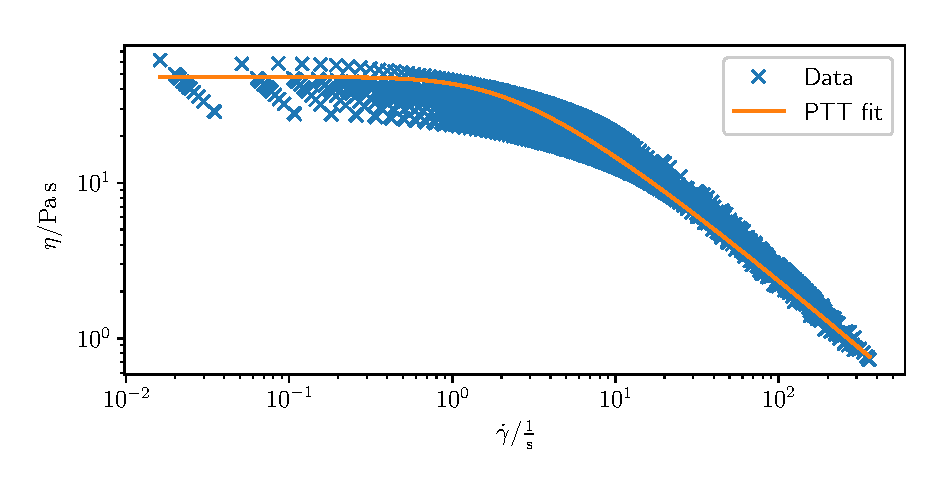
\includegraphics[width=7.8cm]{assets/plots/fit_alginate_eta.eps}
		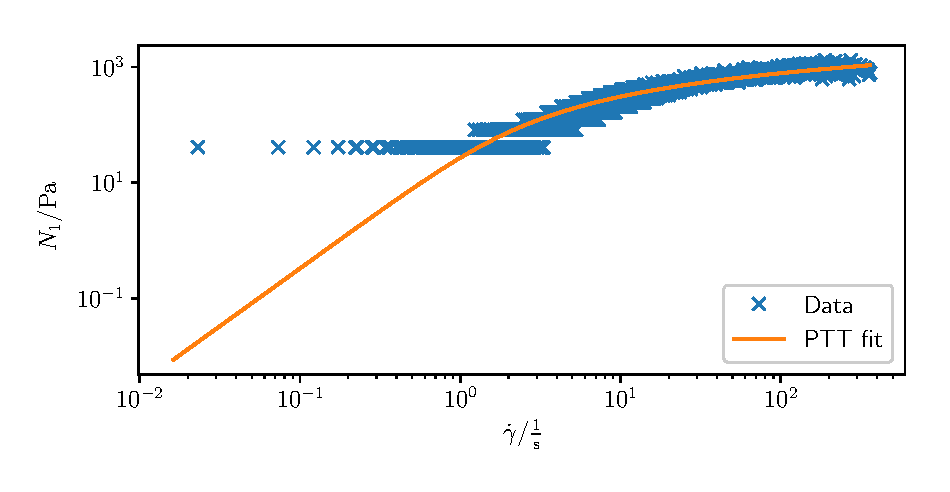
\includegraphics[width=7.8cm]{assets/plots/fit_alginate_N.eps}
%		\adjincludegraphics[trim=0 0 0 0, clip, scale=1]{assets/plots/fit_alginate_eta.eps}
%		\adjincludegraphics[trim=0 0 0 0, clip, scale=1]{assets/plots/fit_alginate_N.eps}
		\caption{Rheology data for alginate solution from 21 measurements of the viscosity (a) and normal stress (b).
				Orange lines show a fit of the PTT rheological model. \SG{ larger font in figures }}
		\label{fig:fit_alginate}
	\end{figure}

The second cell carrier fluid modeled in this work is a methyl cellulose solution which is commonly used in real-time-deformation-cytometry (RT-DC) experiments.
RT-DC experiments allow very high-throughput measurements of cell mechanical properties and have been used successfully for disease detection by screening blood samples.
We extract our data from \cite{buyukurganci2023} where the shear rheology of methyl cellulose was measured using a plate-plate and cone-plate rheometer.
Three concentrations of \SI{0.49}{\percent}, \SI{0.59}{\percent} and \SI{0.83}{\percent} methyl cellulose in PBS were investigated and their rheology is shown in figure~\ref{fig:fit_mc}.
Even at the highest concentration the zero-shear viscosity is two orders of magnitude lower than for the considered alginate solution.
	\begin{figure}[H]
		\centering
		\includegraphics[width=7.8cm]{assets/plots/fit_mc_eta.eps}
		\includegraphics[width=7.8cm]{assets/plots/fit_mc_N.eps}
		\caption{Rheology data of a methyl cellulose solution from \cite{buyukurganci2023}.
				Orange lines show a fit of the PTT rheological model. \SG{ include legend into figure. Maybe give color coding only in caption? }\SG{ larger font in figures }}
		\label{fig:fit_mc}
	\end{figure}
	
\subsection{Fitting data with the PTT model}	

Due to the complexity of viscoelastic fluids, there is an abundance of (semi-)empirical models to describe rheological data.
Common options include the Oldroyd-B \cite{oldroyd1958} and the FENE-P model \cite{bird1980,bird1987}.
The Oldroyd-B model is not appropriate for most real complex fluids as it features a shear-independent viscosity in clear contradiction to the experimental data presented in figures~\ref{fig:fit_alginate} and \ref{fig:fit_mc}.
Although the FENE-P does reproduce shear-thinning, we were not able to obtain a satisfactory fit to our data for alginate and methyl cellulose with physically reasonable values of the model parameters.
The best fit was obtained with the so-called PTT model due to Phan-Thien and Tanner \cite{phan-thien1977,phan-thien1978} which was for explicitly derived for polymer networks in solution and thus appears to capture well the essential physics behind the alginate solution. \SG{ check that these papers have the exponentail version }.

The PTT model is specified by a constitutive equation for the polymer stress $ \ma{\tau}$:
	\begin{equation}
		\overset{\nabla}{\ma{\tau}} = -\xi\left(\ma{\tau}\cdot\ma{D} + \ma{D}\cdot\ma{\tau}\right) - e^{\frac{\epsilon\lambda}{\eta_\text{p}}\Tr\ma{\tau}}\frac{\ma{\tau}}{\lambda} + 2\frac{\eta_\text{p}}{\lambda}\ma{D}
		\label{eq:polymerStress}
	\end{equation}
where $\ma{D}$ is the strain rate tensor. 
The polymer viscosity is denoted $\eta_\text{p}$ and $\lambda$ is the corresponding relaxation time.  \SG{ are they actually independent? }
$\epsilon$ is the so-called extensibility parameter which controls at which shear rates thinning takes place and $\xi$ describes the slip in the polymer network which we will set to zero in the following.
The upper convected derivative is defined as follows:
	\begin{equation}
		\overset{\nabla}{\ma{A}} = \frac{\Dif\ma{A}}{\Dif t} - \left(\left(\nabla\vec{u}\right)^\text{T}\cdot\ma{A} + \ma{A}\cdot\left(\nabla\vec{u}\right)\right)
	\end{equation}
where $\vec{u}$ is the fluid velocity and $\left(\nabla\vec{u}\right)_{ij} = \nabla_i\vec{u}_j$. 
The material derivative is
	\begin{equation}
		\frac{\Dif\ma{A}}{\Dif t} = \frac{\partial\ma{A}}{\partial t} + \vec{u}\cdot\nabla\ma{A}.
	\end{equation}	
Finally, the total fluid stress is the sum of the polymer stress $ \tau $ and a solvent stress $ \tau _ \mathrm{s}$ due to the Newtonian solvent with viscosity $ \eta _ \mathrm{s}$.

For a simple shear flow in the $xy$-plane, an analytical expression for $ \eta $ and $N_1$ is given by \cite{ferras2019} which (with $\xi=0$) reads
	\begin{equation}
		\eta\left(\dot{\gamma}\right) = \frac{\eta_\text{p}}{\exp\left[0.5W_0\left(4\epsilon \mathrm{Wi}^2\right)\right]} + \eta _\mathrm{s} \ma{D}
	\end{equation}
	\begin{equation}
		N_1 = \frac{\eta_\text{p}}{2\epsilon\lambda}W_0\left(4\epsilon \mathrm{Wi}^2\right)
	\end{equation}
where $ \mathrm{Wi} = \lambda \dot{ \gamma  }$ is the Weissenberg number and $W_0$ is the Lambert $W$-function. \SG{ check that $ \eta _ \mathrm{s}$ is correct }
\SG{ I did not find these equations in \cite{ferras2019}? }
Fitting these equations to the rheological data for alginate and methy cellulose leads to satisfactory agreement as shown in figures~\ref{fig:fit_alginate} and \ref{fig:fit_mc}.
In the fit, the solvent viscosity was fixed at $ \eta _ \mathrm{s} = 1 \si{ mPa } \cdot \si{ s }$ as the viscosity of the PBS buffer. \SG{ give ref }
At very high shear rates, the contained polymers are completely stretched and the viscosity asymptotically approaches the solvent values $ \eta _ \mathrm{s}$.
The obtained parameters for alginate are
	\begin{align}
		\eta_\text{p} &= \SI{48.2\pm0.4}{\pascal\second}\\
		\lambda &= \SI{0.343 \pm 0.004}{\second}\\
		\epsilon &= \num{0.545 \pm 0.010}.
	\end{align}
while the parameters for the three concentrations of methyl cellulose are given in table~\ref{tab:MC_parameters}.
	\begin{table}[H]
		\centering
		\begin{tabular}{c|c|c|c}
%			Concentration/\unit{\percent} & $\eta_\text{p}/\unit{\milli\pascal\second}$ & $\lambda/\unit{\milli\second}$ & $\epsilon$ \\
			Concentration/ percent & $\eta_\text{p}/mPas$ & $\lambda/ms$ & $\epsilon$ \\
			\hline
			\num{0.49} & \num{18.7\pm0.4} & \num{0.344\pm0.003} & \num{0.270\pm0.003} \\
			\num{0.59} & \num{32.5\pm0.7} & \num{0.433\pm0.004} & \num{0.365\pm0.004} \\
			\num{0.83} & \num{81\pm2} & \num{0.714\pm0.009} & \num{0.496\pm0.006}
		\end{tabular}
		\caption{Parameters of the PTT modelobtained when fitting the methyl cellulose solutions.}
		\label{tab:MC_parameters}
	\end{table}

We introduce the ratio between the zero-shear and the infinite-shear (i.e.\ solvent) viscosity as 
\begin{align}
	R_ \eta  = \frac{ \eta _ \mathrm{p} } { \eta _ \mathrm{s} }		\label{eq:R_eta}
\end{align}
which will turn out to be an important parameter to determine numerical stability of LB simulations. \SG{ do we actually need a ratio? Since $ \eta _\mathrm{s}$ is probably always water-like, would it not be enough to state whether $ \eta _ \mathrm{p}$ is high or low } \SG{ do we actually show that $R_ \eta  $ determines stability? }
This ratio can in a similar fashion be defined for other models such as FENE-P or the inelastic, but shear-thinning Carreau-Yasuda model \cite{carreau1972, yasuda1979}.
For our alginate solution we obtain $R _ \eta = \num{48.2\pm0.4e3}$, indicating that the solution viscosity at very low shear rates is more than four orders of magnitude larger than the solvent viscosity which represents a severe challenge to standard numerical algorithms.
That this characteristic is not unique to alginate, but is in fact a generic feature of cell carrier fluids used in bioprinting is shown in table~\ref{tab:bioinks} where rheological from various literature sources have been compiled into a single format to determine $ R_ \eta $.
The 0.49 \% methyl cellulose solution used in RT-DC measurements, in contrast, features a much lower value of $R_\eta = \num{18.7\pm0.4}$.
\begin{table}
	\centering
		\begin{tabular}{l|p{3cm}|p{1.5cm}|p{1.5cm}|p{1.5cm}|p{2cm}}
%			Author & Material & $\eta_0/\unit{\pascal\second}$ & $\eta_\infty/\unit{\pascal\second}$ & $R_\eta$ & extracted from \\
			Author & Material & $\eta_0/Pas$ & $\eta_\infty/Pas$ & $R_\eta$ & extracted from \\
			\hline
			Amorim\cite{amorim2021} & pre-crosslinked alginate &  >1e4 & <3e-1 & >3e4 & Fig. 3b \\
			\rowcolor{secondaryBackground}
			Pössl\cite{possl2021} & blend & 3e2 & 1e-4 & 3e6 & Table 4 \\
%			Paxton\cite{paxton2017} &Nivea Creme\n Alginate& 1e5\n5e4 & <1\n<5e1 & >1e5\n>1e3 & Fig. 4b \\
			Paxton\cite{paxton2017} & Alginate& 5e4 & <5e1 & >1e3 & Fig. 4b \\
			\rowcolor{secondaryBackground}
			O'Connell\cite{oconnell2020} & pluronic F-127 & >1e6 & <8 & > 2e5 & Chapter 7 Fig. 13 \\
		\end{tabular}
	\caption{Compilation of literature data on typical bioinks showing that a very viscosity ratio $ R_ \eta $ is a generic feature of these liquids. }
	\label{tab:bioinks}
\end{table}

	
%%
%% LBM
%%	
	
\section{Existing LBM methods}

Since the early days of LBM methods for viscoelastic fluids have been developed. 
Keeping in mind our target geometries, we focus here on three dimensional formulations.
The first approaches avoided an explicit modeling of a viscoelastic constitutive equation and simply modified the LB collision operator to obtain a fluid obeying Jeffery's viscoelastic model \cite{lallemand2003}. \SG{ can we say more about Jeffery? Why is it bad? Is it shear-thinning? }
More advcanced approaches include the work of Onishi \textit{et al.} \cite{onishi2005, onishi2006} who considered a non-shear-thinning Oldroyd-B model using a microscopic Fokker-Planck equation for the polymer dumbbells. 
The work of \cite{malaspinas2010} and \cite{ma2020} considered in addition the FENE-P model solving the advection part of the model using a second LBM running in parallel to the Navier-Stokes LBM while \cite{wang2020} used this approach for the Oldroyd-B model.
Later, hybrid schemes coupling an LB solver for the solvent to a finite-difference \cite{gupta2015_2, gupta2015, gupta2016} or finite-volume \cite{kuron2021} scheme for the polymer stress (or, alternatively, the polymer conformation) tensor were introduced.
To improve numerical stability, some authors propose the inclusion of an artificial diffusivity \SG{ cite }, which introduces a small error compared to the analytical solution of the constitutive equation. 
Coupling of the resulting polymer stress to the Navier-Stokes LBM can be achieved via the inclusion of point forces or via a modification of the equilibrium populations.
A recent comparison in 2D found that the former in general leads to higher stability \cite{dzanic2022}.

The stable range of Weissenberg numbers covered by existing methods is up to $ \mathrm{Wi}  \approx  10$ for the method of \cite{malaspinas2010} and up to $ \mathrm{Wi}  \approx 100$ in \cite{gupta2015,ma2020,gupta2016}.
However, another stability criterion, which is often overlooked is the viscosity ratio $ R_ \eta $ as defined in XX. 
Existing methods often stay at or below $R_\eta = 1$\cite{gupta2015,onishi2006,wang2020,su2013_2,gupta2015_2}, while the ones trying higher ratios report being limited below $R_\eta = 10$\cite{malaspinas2010,ma2020,kuron2021} due to stability issues. 
The details are listed in table~\ref{tab:viscRatio}.
Comparing to the rheological data presented in figures~\ref{fig:fit_alginate} and \ref{fig:fit_mc}, we conclude that existing LB methods appear to be appropriate only for relatively dilute solutions and in particular do not cover the viscosity ratio required by these technologically important cell carrier fluids.
We therefore set out to develop a novel viscoelastic LB scheme which we will present in the next section. 

\begin{table}
\begin{center}
			\begin{tabular}{l|r|r|l}
				Author & max(Wi) & max($R_\eta$) & $R_\eta$ estimation \\
				\hline
				Malaspinas\cite{malaspinas2010} & 10 & 9 & In 4.3: $R_\nu = \num{0.1}$ \& equation (38) \\
				\rowcolor{secondaryBackground}
				Gupta\cite{gupta2015} & 100 & 0.7 & In IV.B: $\frac{\eta_\text{p}}{\eta_\text{A} + \eta_\text{p}} = \num{0.4}$ \\
%				Dzanic\cite{dzanic2022} & 10 & 0.5 & In 4.1: $\beta = \frac{\nu_\text{p}}{\nu_\text{s}} = \num{0.5}$ \\
				Ma\cite{ma2020} & 100 & 9 & In 4.1: $\beta = \frac{\mu_\text{s}}{\mu_\text{s} + \mu_\text{p}} = \num{0.1}$ \\
				\rowcolor{secondaryBackground}
				Onishi\cite{onishi2006} & ? & 1 & In 3.1: $\beta = \frac{\mu_\text{p}}{\mu_\text{s} + \mu_\text{p}}$ \& Table 1: $\beta=\num{0.5}$ \\
				Wang\cite{wang2020} & \glqq up to O(1)\grqq & 5 & In II: $\eta_\text{p} = c\eta_\text{s}$ \& FIG. 9: $c = \num{5}$\\
				\rowcolor{secondaryBackground}
%				Dzanic\cite{dzanic2022_2} & 10 & 9 & In 5.1: $\beta = \frac{\nu_\text{s}}{\nu_\text{s} + \nu_\text{p}}$ \& In 5.1.2: $\beta = \num{0.1}$ \\
				Su\cite{su2013_2} & 10 & 1  & In II: $\beta = \frac{\eta_\text{s}}{\eta_\text{s} + \eta_\text{p}}$ \& In IV.A: $\beta = \num{0.5}$ \\
				Gupta\cite{gupta2015_2} & ? & 0.7 & In 2: $\frac{\eta_\text{p}}{\eta_\text{d}} = \num{0.4}$ \& $\eta_\text{d} = \eta_\text{A} + \eta_\text{p}$ \\
				\rowcolor{secondaryBackground}
				Kuron\cite{kuron2021} & 1 & 9 & In 4.1: $\beta = \num{0.9}$ \& equations (14) \& (15) \\
				Gupta\cite{gupta2016} & 80 & 0.7 & In 3: $\frac{\eta_\text{p}}{\eta_\text{c,d} + \eta_\text{p}} = \num{0.4}$ \\
				\rowcolor{secondaryBackground}
				Onishi\cite{onishi2005} & 1000 & 1 & In 3.2: $\frac{\eta_\text{p}}{\eta_\text{s}} = \num{1}$ \\
			\end{tabular}
		\end{center}

\caption{Covered ranges of $ \mathrm{Wi}$ and $ R_ \eta $ for existing 3D LB methods.}
\end{table}



%%
%% Our method
%%
	
\section{Numerical methods}
\label{sec:Methods}

Our algorithm contains a Lattice-Boltzmann solver for the Navier-Stokes equations of the solvent, a finite-volume solver for integrating the polymer stress and finally our newly developed viscosity shuffling method.

\subsection{Lattice-Boltzmann for Navier-Stokes}

The Lattice-Boltzmann method (LBM) has become a standard tool in numerical fluid mechanics \cite{Kruger_book} and we therefore describe it here only very briefly.
We use a D3Q19 lattice in full three dimensions together with a single relaxation time collission operator.
Our implementation is based on FluidX3D which has been extensively used and validated in earlier publications \cite{Lehmann.20229da}.
The core of the algorithm is implemented in OpenCL and thus capable of running on GPUs from different vendors.
Boundaries are modeled using the half-way bounce back algorithm. 
\SG{ and inflow/outflow: give details }

Physical units are mapped to lattice units to obtain a dimensionless relaxation time of 1.
The employed lattice dimensions vary for the different applications and are specified below. \SG{ to do }
To drive the flow, we use either a constant body force (modeling a physical pressure gradient) or inflow-outflow boundaries as specified in the different application scenarios below. \SG{ check, specify }

\subsection{Finite-volume for polymer stress }

The spatio-temporal dynamics of the polymer stress $ \ma{ \tau  }$ is given by equation~(\ref{eq:polymerStress}) in the form of an advection-reaction equation.
We solve this equation with a finite-volume running in parallel (with identical time step) with the LBM solver.
Advection is handled using the corner transport upwind scheme \cite{kuron2021}.
At the walls, a zero-flux boundary condition for the stress is used.
The source terms are integrated using the Euler method. 

To include the polymer stress into the LBM, we use the stress coupling scheme according to Dzanic et al.\cite{dzanic2022_2, gupta2015, onishi2006}. 
For this, ... \SG{ give some more details, especially since we do SRT }.
\SG{ also include inflow/outflow BCs }
\SG{ do you advect polymer stress or polymer conformation? }

The total stress experienced by the fluid ($\ma{\sigma}$) is then \cite{onishi2006}:
	\begin{align}
		\ma{\sigma} &= 2\eta_\text{s}\ma{D} + \ma{\tau} 		\label{eq:totalStress}
	\end{align}
	


\subsection{Novel viscosity shuffling}\label{sec:shuffling}

The key difficulty for simulating many realistic viscoelastic fluids is the unbalance between the viscous stress of the solvent and the polymer stress.
While the former is handled efficiently and reliably by the LBM streaming-collision scheme, the latter enters the LB equations as an additional source term.
The relative magnitude of the two terms is given by the viscosity ratio $R_ \eta $ as defined in equation~\ref{eq:R_eta} which for many situations is of the order of $10^2-10^4$ (see figure~\ref{fig:fit_alginate} and \ref{tab:bioinks}).
The key idea of our scheme is to artificially increase the LBM viscous stress while at the same time reducing the polmer stress by the same amount.
Starting from equation~\ref{eq:totalStress}, we write
\begin{align}
	\ma{\sigma} &= 2\eta_\text{s}\ma{D} + \ma{\tau}_\text{shuffle} + \ma{\tau} - \ma{\tau}_\text{shuffle}	
\end{align}
with the transfered (''shuffled'') stress
\begin{align}
	\ma{ \tau }_ \mathrm{shuffle} = 2 \alpha _ \mathrm{s} \eta _ \mathrm{p} \ma{D}
\end{align}
containing an arbitrary parameter $0 < \alpha _ \mathrm{s} < 1$.
Finally, this results in
\begin{align}
	\ma{ \sigma } &=  2\left(\eta_\text{s} + \alpha_\text{s}\eta_\text{p}\right)\ma{D} + \left(\ma{\tau} - 2\alpha_\text{s}\eta_\text{p}\ma{D}\right).
\end{align}
In practice, the shuffling parameter $ \alpha _ \mathrm{s}$ is chosen before the start of the simulation.
The LBM solver is run with $\eta_\text{s} + \alpha_\text{s}\eta_\text{p}$ as its viscosity while from the polymer stress determined by equation~\ref{eq:polymerStress} the amount $\alpha_\text{s}\eta_\text{p} \ma{D}$ is subtracted at every time step before it is coupled into the LBM.

Using this procedure, we balance the stress contributions of the LB and the polymer components which vastly improves numerical stability.
We emphasize that, in contrast to other remedies such as adding artificial diffusivity \SG{ refs }, our viscosity shuffling algorithm is mathematically exact and does not affect the physics of the simulated system.
\SG{ re-include effective $R_ \eta $? }
%	In terms of stability, we could define an effective $R_\eta$, calculated from the stress contributions as follows.
%	\begin{equation}
%		R_{\eta\text{, eff}} = \frac{\eta_\text{p}-\alpha_\text{s}\eta_\text{p}}{\eta_\text{s} + \alpha_\text{s}\eta_\text{p}} = \frac{1-\alpha_\text{s}}{\frac{\eta_\text{s}}{\eta_\text{p}} + \alpha_\text{s}} = \frac{1-\alpha_\text{s}}{1 + \alpha_\text{s}R_{\eta}}R_{\eta} \overset{\alpha_\text{s}R_{\eta}\gg1}{=} \frac{1-\alpha_\text{s}}{\alpha_\text{s}}
%	\end{equation}
	%Given $\alpha_\text{s}$ is large enough, arbitrary $R_{\eta\text{, eff}}$ can be reached, bringing the simulation within the range, that is stable with current methods, and thus arbitrary $R_{\eta}$ become stable. 
The only trade-off of our viscosity shuffling scheme is that the increased LB viscosity decreases the LB time step if the lattice relaxation time is maintained at its optimal value of 1.
In the following section we validate this novel approach against analytical solutions for realistic parameters and compare its accuracy to existing algorithms.

%%
%% Validation and accuracy
%%
	
\section{Validation and accuracy}
	
To validate our viscosity shuffling algorithm and to assess its accuracy, we compare the velocity fields to semi-analytical solutions in plane and cylindrical Poiseuille flow.
For the PTT model given in equation~(\ref{eq:polymerStress}) with an additional solvent stress contribution as in equation~(\ref{eq:totalStress}) a full analytical solution is not known for the considered geometries.
Based on the work of \cite{oliveira1999} we derive a semi-analytical solution in Appendix~\ref{app:PTT}.

We start by simulating the alginate and 0.49\% methyl cellulose solutions with a viscosity ratio $R_ \eta = 48 \cdot 10 ^3$ and $R_ \eta = 18.7$, respectively, in 2D planar Poiseuille flow.
In physical units the channel has a height of \SI{20}{\micro\meter} which are discretized with \SG{ XX } LBM nodes.
For the viscosity shuffling, we set $ \alpha _ \mathrm{s} = XX$.
Along the flow direction, the channel is periodic and the flow is driven by a pressure gradient of \SI{-1e7}{\pascal\per\meter}. \SG{ pressure for MC? }
The velocity field is initialized with zero.
For methyl cellulose, we simulate the full temporal evolution with the polymers starting in the unstretched configuration.
In the case of alginate, we speed up the convergence and start from a situation in which the polymers are pre-stretched \SG{ give details }.
After \SG{ XX } LBM time steps corresponding to \SG{ XX } of physical time, the simulation is stopped and the flow field $u(y)$ is compared to the semi-analytical solution.
As shown in figure~\ref{fig:2DAlginateU}, very good agreement is found.
For a quantitative assessment, we compute the L2 error as
	\begin{equation}\label{eq:l2error}
		E_\text{u} = \frac{1}{u_\text{max}}\sqrt{\frac{1}{N}\sum\abs{u_\text{simulation}-u_\text{theory}}^2}.
	\end{equation}
The spatially resolved errors are shown in figure~\ref{fig:2DAlginateErr} in the appendix.
Averaging over the channel diameter, we obtain an L2 error of \num{9e-4} and \SG{ XX } for alginate and methyl cellulose, respectively..	

	\begin{figure}[H]
		\centering
		\adjincludegraphics[trim=0 0 0 0, clip, scale=0.5]{assets/plots/2DAlginateU.eps}
		\adjincludegraphics[trim=0 0 0 0, clip, scale=0.5]{assets/plots/2DParameterStudyUWorst.eps}
		\caption{(a) Velocity profile of alginate in planar channel flow. \SG{use $y$ instead of $r$ in 2D}. 
		The time evolution of the center-line velocity when starting from a pre-stretched configuration (see main text) is shown in the inset.
		(b) Velocity profile for methyl cellulose.}
		\label{fig:2DAlginateU}
	\end{figure}
	
We now proceed to evaluate the viscosity shuffling method for a cylindrical pipe flow.
The semi-analytical solution for this situation can be derived in a similar fashion as for the planar case and is given in appendix ~\ref{app:semianalyticalPoiseuille}.
Numerically, the cylindrical sitation is slightly more complex due to discretization errors (''staircase effect'') when mapping the rounded channel walls onto the rectilinear LBM grid \cite{Lehmann.20229da}.
We use the same material parameter set as above, but double the pressure gradient to \SG{ XX }. \SG{ why? }
The channel has a diameter of \SG{ XX } and is discretized with 41 lattice points.
Again, we initialize the polymers in the unstretched state for methyl cellulose and in the stretched state for alginate.
The resulting velocity profile can be seen in figure \ref{fig:3DAlginateU} and shows almost equally good agreement as for the planar case with an L2 error of \num{0.014}.
The spatially resolved error shows that this larger average is indeed mainly attributable to the staircase effect as the error near the walls increases significantly.



	\begin{figure}[H]
		\centering
		\adjincludegraphics[trim=0 0 0 0, clip, scale=0.5]{assets/plots/3DAlginateU.eps}
		\adjincludegraphics[trim=0 0 0 0, clip, scale=0.5]{assets/plots/3DParameterStudyUWorst.eps}
		\caption{(a) Velocity profile of alginate in cylindrical channel flow. 
		The time evolution of the center-line velocity when starting from a pre-stretched configuration (see main text) is shown in the inset.
		(b) Velocity profile for methyl cellulose.}
		\label{fig:3DAlginateU}
	\end{figure}






	%We use richard/master fe0fc04115b9b6ea6628bcc6cb6593d3f72ac0ea (2023-11-05)
	\subsection{Comparison with literature}
	Malaspinas et al.\cite{ma2020} provide a detailed validation and claim very high accuracy. Therefore, we pick this as a comparison. We aim at the reproduction of figures 17 and 18 from said paper. We calculate this 2D flow in 3D as the viscoelastic algorithm has not been validated for 2D velocity sets. Otherwise, the geometry is identical. It is not entirely clear to us, how they define typical scales. We define the typical velocity as the maximum velocity, as is likely done in the paper. The typical length, we set as half of the channel width. We define the typical shear rate as typical velocity divided by typical length. We set $\eta_\text{s} = \SI{1}{\milli\pascal\second}$ as the paper only gives ratios, and it probably does not matter here. Nevertheless, our lattice units do not line up exactly with those from Malaspinas, as our viscosity is different due to the shuffling.
	%Beware equation 61 in the paper is wrong. It should have an 8 instead of the 4.
	The parameters from the paper ($R_\nu$, $Wi$ and $N$) are varied as in the paper. 
	\begin{figure}[H]
		\centering
		\adjincludegraphics[trim=0 0 0 0, clip, scale=1]{assets/plots/malaspinas2010.eps}
		\caption{Double logarithmic plot of the L2 error as defined in equation \ref{eq:l2error} from Malaspinas et al.\cite{malaspinas2010} (dots) compared to our algorithm (x) as a function of grid resolution.}
		\label{fig:malaspinas2010}
	\end{figure}
	As can be seen in figure \ref{fig:malaspinas2010}, our results notably do not depend on the Weissenberg Number. While our error decreases with N with a constant power, Malaspinas et al. see diminishing returns. While these results are excellent, the error in our implementation seemingly is still dependent on the viscosity ratio. As the error is still small using our alginate parameters (see section \ref{sec:channelFlow}), this effect is irrelevant. With this, one can see, that we are not only capable to simulate parameters not yet accessible, but our implementation is also better for the parameters used in literature. Knowing our simulations to be good we in the following show results for interesting systems, that are not analytically solvable.
	
	
	
	
	
	
	
	
	
	
%	For pressure gradient driven channel and pipe geometries, the analytical solution is as follows.
%	\begin{equation}
%		u\left(r\right) = \frac{Gl^2}{2^{j+1}\eta_\text{p}}\left(e^\frac{R^2}{l^2}-e^\frac{r^2}{l^2}\right)
%	\end{equation}
%	Where $u\left(r\right)$ is the radius dependent velocity, $G = -\partial_xp$ is the pressure gradient in the direction of the pipe and $l$ is a constant defined as follows.
%	\begin{equation}
%	l^2 = \frac{2^{2j-1}\eta_\text{p}^2}{\epsilon\lambda^2G^2}
%	\end{equation}
%	The index $j$ gives the solution for the channel for $j=0$ and the pipe for $j=1$.
%	
%	We need this solution to compare to literature. However, this solution does not include $\eta_\text{s}$, which is required in general. With the inclusion of the solvent viscosity an analytical solution can no longer be found and the use of a semi-analytic solution is required (for details see appendix \ref{app:PTT}).
%	In the following we compare results for channel and pipe flow to these equations for realistic parameters. Afterward we compare the accuracy of our simulation algorithm against literature.
	
	


	
	
%%
%% Example applications
%%	
	
\section{Example applications}

To illustrate the use of viscosity shuffling in realistic applications, we study three typical experimentally relevant situations.
For ease of comparison, we use the 0.49\% methyl cellulose in all three situations.

The first application stems from bioprinting where the bioink is pushed through a conical nozzle \SG{ ref }.
The nozzle radius is \SI{1.8}{\milli\meter} at the inlet and \SI{200}{\micro\meter} at the outlet. 
The nozzle has a length of \SI{18}{\milli\meter}.
Due to the difference in inlet/outlet radii, the system cannot be modeled with periodic boundary conditions and we use inflow-/outflow boundary conditions as described in section~\ref{sec:Methods} instead.
The required values for velocity and polymer conformation are obtained from simulations of pipes of the respective radii and a fixed volume flow of $\approx\SI{3}{\micro\liter\per\second}$.
The resulting flow field can be seen in figure \ref{fig:Nozzle_v}~(a). 
To quantify the total stress as a single number, we use the von Mises stress which is defined as \cite{Mueller.2023}: 
\begin{align}
	\sigma _ \mathrm{vM} = \sqrt{ \frac{ 1 } { 2 } \left[ \left( \sigma _1 - \sigma _2 \right)^2 + \left( \sigma _2 - \sigma _3 \right)^2 + \left( \sigma _3 - \sigma _1 \right)^2 \right]}.
\end{align}
It can be seen that the highest stresses aries at the nozzle exit in direct vicinity to the wall.
This means that even for fast flows,  cells flowing close to the center experience less stress than cells flowing near the walls in agreement with earlier results in Newtonian fluids \cite{Mueller.2023}.
	\begin{figure}[H]
		\centering
		\adjincludegraphics[trim=0 0 0 0, clip, scale=0.5]{assets/plots/Nozzle_v.eps}
		\adjincludegraphics[trim=0 0 0 0, clip, scale=0.5]{assets/plots/Nozzle_sigma_vM.eps}
		\caption{Velocity profile (a) and von Mises stress (b) for methyl cellulose in a conical nozzle as used for bioprinting. \SG{ draw nozzle contour with black lines }}
		\label{fig:Nozzle_v}
	\end{figure}

% nozzle: We use richard/vtk 4dbc4d379842c538f084e68a5dcfe2555a674495 (2024-01-09)
% shear: 	We use richard/vtk 4dbc4d379842c538f084e68a5dcfe2555a674495 (2024-01-09)
% RT-DC: We use richard/master fe0fc04115b9b6ea6628bcc6cb6593d3f72ac0ea (2023-11-05)
	
Our next example is the RT-DC geometry in which cells from a reservoir are squeezed through a narrow observation channel \cite{Toepfner.2018, Fregin:2019gx} with a square cross-section of 20x20 $\mu m$.
For this simulation we use periodic boundary conditions and a constant body force corresponding to a pressure gradient of \SI{1e7}{\pascal}. 
In figure~\ref{fig:RT-DC}, we show the velocity profile and the shear component of the stress which is the relevant component if a local shear viscosity is to be defined.
There are three qualitative differences compared to a purely viscous fluid. 
Directly after the inlet we find a region of low stress. 
Due to the fast advection, the polymers, despite being inside the constriction, have not reacted to the increased fluid stress yet.
Similarly, directly after the constriction, the high stress inside the observation channel persists over a certain distance that is needed for the polymer stress to decay.

 
 	\begin{figure}[H]
		\centering
		\adjincludegraphics[trim=0 0 0 0, clip, scale=0.5]{assets/plots/RT-DC_v.eps}
		\adjincludegraphics[trim=0 0 0 0, clip, scale=0.5]{assets/plots/RT-DC_tau.eps}
		\caption{Velocity profile (a) and shear stress (b) for methyl cellulose in a typical RT-DC geometry. \SG{ draw channel contour with black lines }
		\SG{ change to von Mises instead of $ \tau _{ 12 }$? }}
		\label{fig:RT-DC}
	\end{figure}

\SG{ decide whether we want to show a viscosity plot and remove or leave this part:
If one would divide the stress in these two regions by the strain rate in an attempt to obtain a viscosity one would find an extremely low and an extremely high viscosity respectively. Depending on the exact parameters \glqq viscosities\grqq{ }can be reached that cannot be obtained through rheological measurements with the fluid. Meaning these viscosities are not valid. This is even clearer along the walls directly after the outlet. Here the viscosites obtained in this manner become negative. This shows the breakdown of the viscosity interpretation in viscoelastic cases and signifies the regions of interesting behavior. This also shows why viscoelastic simulations cannot always be replaced by shear thinning models and should be considered despite the high computational cost. }

With the third example we demonstrate the versatility of our approach which allows easy coupling to other LBM extensions such as the immersed-boundary method.
Here, we include a homogeneously elastic particle as a simple, yet reasonably accurate, model for the mechanics of a living, biological cell \cite{Wohlrab.2023}.
Coupling to the LBM solver is achieved with the immersed-boundary method as described in earlier publications \cite{Mueller.2021}.
For simplicity, we consider the viscoelastic fluid inside and outside of the cell to be identical.
The cell is initially spherical with a radius of \SI{6}{\micro\meter} and possesses Youngs Modulus of \SI{100}{\pascal} and a Poisson ratio of \SG{ XX }.
It is placed into a shear flow with a shear rate of \SI{400}{\per\second} where the cell quickly reaches a steady state in which it deforms into a tank-treading ellipsoid.
For the discretization of the cell we use \SG{ xx } tetrahedrons and a radius of \SG{ xx } lattice units.
The lattice with a resolution of \num{100} lattice points is chosen significantly bigger than the cell to assure negligible impact of the walls. 
The lattice is periodic in $x$ and $z$ direction.
At the edges of the simulation box in $y$ direction Dirichlet boundary conditions are imposed.
	
In the von Mises stress seen in figure \ref{fig:cellInShear_vM} the effect of the cell is clearly visible. 
We observe four distinct regions of high stress radiating outwards from the cell body.
These are particularly pronounced along the longest axis of the deformed cell. 
\SG{ connect to the ''viscoelastic wings'' paper }

	\begin{figure}[H]
		\centering
		\adjincludegraphics[trim=0 0 0 0, clip, scale=1]{assets/plots/cellInShear_sigma_vM.eps}
		\caption{The von Mises stress around a cell in shear flow.}
		\label{fig:cellInShear_vM}
	\end{figure}	
	
%%
%% Conclusion
%%	
	
\section{Conclusion}


	\newpage
	\printbibliography[heading=bibintoc]
	
%%
%% Appendix
%%	
	
	\appendix
	\appendixpage
	
%%
%% Exp protocol
%%	
	
\section{Rheology measurements of alginate solutions}	

\SG{ Tomasz should extend this paragraph }
The solutions used here are 4\% by weight of DuPont VIVAPHARM Alginate PH176 in PBS. 
The measurements were done using a plate-plate rheometer. 
Data is agglomerated from 21 independent measurements.
The first normal stress difference $N_1$ is calculated from the measured normal force using the following equation\cite{kulicke1977}.
	\begin{equation}
		N_1 = \frac{2F}{\pi R^2} + \frac{3}{20}\rho\omega^2R^2
	\end{equation}
	Where $F$ is the measured normal force, $R$ is the radius of the rheometer, $\rho$ is the density of the fluid and $\omega$ is the angular velocity of the rheometer. The second term is usually omitted and as we found it to matter little, and as the quality of the data we have available is too limited to warrant such detailed corrections, we also choose to omit it. A cone-rheometer would be preferred here, but as $N_2 = 0$ for PTT with $\xi = 0$, the difference is negligible.
	
	
	\section{Implementation of constitutive equations}\label{app:implementation}\todo{Note available analytical solutions}
	There is a large amount of viscoelastic models. It is also common to extend these to create new models. As Oliveira shows\cite{oliveira2009} many of these can be expressed to a common form and thus actually are variants of a common idea. This allows both to easily find new models and implement them. In the following polymer contributions $\ma{\tau}$ of the models we have currently implemented are described. For notation, we mostly follow close to Oliveira\cite{oliveira2009}.
	\parab{Implementation}
	The actual implementation uses tensors related to $\tau$ to unify the calculations as much as possible. We denote these tensors as $\ma{A}$ and give the relation for each model. Whenever we explicitly need $\ma{\tau}$, we convert it. For Oldroyd-B this does not seem necessary and might even be slightly detrimental to performance. However, such a replacement simplifies the constitutive equation for FENE-P significantly and doing it for the other models as well allows a unified code with little adaptation for each model. It also makes the equations easier to understand and analyze. We stick with $\ma{A}$ as the Tensor containing the stress information, although its meaning is different for the different models listed here. This way, it can be seen, that all the models listed here can be brought to the common form listed below.
	\begin{equation}
		\frac{\partial\ma{A}}{\partial t} + \vec{u}\cdot\nabla\ma{A} = \left(\left(\nabla\vec{u}\right)^\text{T}\cdot\ma{A} + \ma{A}\cdot\left(\nabla\vec{u}\right)\right)+\ma{S}_\text{R} + 2\ma{D}
	\end{equation}
	Where $\ma{S}_\text{R}$ is a model-dependent term. In the following only this will be specified as all other terms are the same for all models. The second term on the left-hand side is handled via CTU, the rest is Euler-integrated.
	
	\subsection{Oldroyd-B}
	This model was originally developed by Oldroyd\cite{oldroyd1958}. The constitutive equation reads as follows.
	\begin{equation}
		\overset{\nabla}{\ma{\tau}} = -\frac{\ma{\tau}}{\lambda} + 2\frac{\eta}{\lambda}\ma{D}
	\end{equation}
	$\lambda$ is the polymer relaxation time and $\eta$ is the polymer viscosity. This viscosity also defines the magnitude of the elastic forces. Both these parameters also appear in the other models. We usually do not use this model, as it is not shear thinning.
	\parab{Implementation}
	\begin{equation}
		\ma{S}_\text{R} = -\frac{\ma{A}}{\lambda}
	\end{equation}
	\begin{equation}
		\ma{\tau} = \frac{\eta}{\lambda}\ma{A}
	\end{equation}
	
	\subsection{FENE-P}\todo{cite oliveira for theory}\todo{a lot more detail can be found in my dedicated FENE-P repo -> include derivation?}
	This model was originally developed by Bird\cite{bird1980}\cite{bird1987}. It can be viewed as an Extension of the Oldroyd-B by limiting the polymers to finite extensibility. It has particularly many derivatives. Its constitutive equation reads as follows.
	\begin{equation}
		\overset{\nabla}{\ma{\tau}} = -Z\frac{\ma{\tau}}{\lambda} + \left(\ma{\tau}+(1-e b)\frac{\eta}{\lambda}\uT\right)\frac{\Dif\ln Z}{\Dif t} + 2(1-eb)\frac{\eta}{\lambda}\ma{D}
	\end{equation}
	With the extensibility parameter b, $e = \frac{2}{b\left(b + 2\right)}$ and
	\begin{equation}
		Z = 1 + \frac{3}{b}\left(\frac{b}{b + 2}+\frac{\Tr\ma{\tau}}{3\frac{\eta}{\lambda}}\right)
	\end{equation}
	Note, that the sign of $\ma{\tau}$ differs from Birds formulation. Also, the relation $nk_\text{B}\theta = \frac{\eta}{\lambda}$ has already been used to avoid introducing additional parameters. Particularly for large shear rates, it is numerically possible, that the polymer exceeds its maximal extensibility. If it is extended beyond the maximum the equations cause it to extend further, making this model unstable for high shear rates. Even with the decomposition proposed by Dzanic\cite{dzanic2022}, we were not yet able to get it stable. Thus, it is currently unused.
	\parab{Implementation}
	\begin{equation}
		\ma{S}_\text{R} = \frac{\Tr\ma{A}\uT + \left(b + 2\right)\ma{A}}{\lambda\frac{b+2}{b+5}\left(\Tr\ma{A}-b-2\right)}
	\end{equation}
	\begin{equation}
		\ma{\tau} = \frac{\eta}{\lambda}\frac{b}{b+2-\Tr\ma{A}}\left(\ma{A}+\frac{\Tr\ma{A}}{b+2}\uT\right)
	\end{equation}
	This seems complicated, but removes the highly problematic $\frac{\Dif\ln Z}{\Dif t}$ term, which causes issues in implementation details.
	
	\subsection{PTT}
	Originating from Phan-Thien and Tanner\cite{phan-thien1977} it was soon after slightly extended by Phan-Thien\cite{phan-thien1978} to the exponential form we use. There is also an even more general form from Ferrás\cite{ferras2019}, which due to its use of the Gamma function is hard to implement on GPUs. The constitutive equation reads as follows.
	\begin{equation}
		\overset{\nabla}{\ma{\tau}} = -\xi\left(\ma{\tau}\cdot\ma{D} + \ma{D}\cdot\ma{\tau}\right) - e^{\frac{\epsilon\lambda}{\eta}\Tr\ma{\tau}}\frac{\ma{\tau}}{\lambda} + 2\frac{\eta}{\lambda}\ma{D}
	\end{equation}
	Where $\epsilon$ and $\xi$ are additional parameters related to the network this model is supposed to model. For our polymer solutions $\xi$ is always (effectively) zero.
	\parab{Implementation}
	\begin{equation}
		\ma{S}_\text{R} = -\xi\left(\ma{A}\cdot\ma{D} + \ma{D}\cdot\ma{A}\right) - e^{\epsilon\Tr\ma{A}}\frac{\ma{A}}{\lambda}
	\end{equation}
	\begin{equation}
		\ma{\tau} = \frac{\eta}{\lambda}\ma{A}
	\end{equation}

	\section{FENE-P}\label{app:FENE-P}
	\todo{stability issue, fitting parameter, see fenep repo}
	
%%
%% Semi-analytical
%%	
	
\section{Semi-analytical solution for Poiseuille flows of PTT fluids with solvent viscosity}
\label{app:semianalyticalPoiseuille}
Our derivation is analogous to Oliveira\cite{oliveira1999}. To account for the added viscous stress due to $\eta_\text{s}$, equilibrium is reached at lower polymer stresses. Therefore, Oliveiras equation (7) needs to be modified as follows.
	\begin{equation}
		\tau_{xy} = \partial_xp\frac{r}{2^j} - \eta_\text{s}\dot{\gamma}
	\end{equation}
	Where the second term is added due to the presence of the solvent viscosity. This term also propagates to Oliveiras equation (9) as follows.
	\begin{align}
		\dot{\gamma} &= f\left(\frac{2\lambda}{\eta_\text{p}}\left[\partial_xp\frac{r}{2^j} - \eta_\text{s}\dot{\gamma}\right]^2\right)\frac{1}{\eta_\text{p}}\left(\partial_xp\frac{r}{2^j}-\eta_\text{s}\dot{\gamma}\right)
		\intertext{This cannot be integrated as easily as without $\eta_\text{s}$, and is only solvable semi-analytically.}
		1 &= f\left(\frac{2\lambda}{\eta_\text{p}}\left[\partial_xp\frac{r}{2^j} - \eta_\text{s}\dot{\gamma}\right]^2\right)\frac{1}{\eta_\text{p}}\left(\partial_xp\frac{r}{2^j\dot{\gamma}}-\eta_\text{s}\right)
	\end{align}
	For the exponential version of PTT $f$ is defined as follows.
	\begin{equation}
		f\left(\Tr\ma{\tau}\right) = \exp\left(\frac{\epsilon\lambda}{\eta_\text{p}}\Tr\ma{\tau}\right)
	\end{equation}
	This can be inserted in the above equation.
	\begin{align}
		1 &= \exp\left(\frac{2\epsilon\lambda^2}{\eta_\text{p}^2}\left[\partial_xp\frac{r}{2^j} - \eta_\text{s}\dot{\gamma}\right]^2\right)\frac{1}{\eta_\text{p}}\left(\partial_xp\frac{r}{2^j\dot{\gamma}}-\eta_\text{s}\right) \\
		0 &= \frac{2\epsilon\lambda^2}{\eta_\text{p}^2}\left[\partial_xp\frac{r}{2^j} - \eta_\text{s}\dot{\gamma}\right]^2 - \ln\eta_\text{p} + \ln\left(\partial_xp\frac{r}{2^j\dot{\gamma}}-\eta_\text{s}\right) \\
		0 &= 2\epsilon\lambda^2\dot{\gamma}^2\left[\partial_xp\frac{r}{2^j\dot{\gamma}\eta_\text{p}} - \frac{\eta_\text{s}}{\eta_\text{p}}\right]^2 + \ln\left(\partial_xp\frac{r}{2^j\dot{\gamma}\eta_\text{p}}-\frac{\eta_\text{s}}{\eta_\text{p}}\right) \\
		0 &= 2\epsilon\lambda^2\dot{\gamma}^2\left[\partial_xp\frac{r}{2^j\dot{\gamma}\eta_\text{p}} - \frac{\eta_\text{s}}{\eta_\text{p}}\right]^2 + \ln\left(\partial_xp\frac{r}{2^j\dot{\gamma}\eta_\text{p}}-\frac{\eta_\text{s}}{\eta_\text{p}}\right)
		\intertext{This has the following form}
		0 &= ab^2 + \ln b
	\end{align}
	This can be solved using the Lambert W function as follows.
	\begin{align}
		b &= -\sqrt{\frac{W_0\left(2a\right)}{2a}}
		\intertext{Resolving for $r$ yields the following.}
		r &=  \frac{2^j\eta_\text{s}}{\partial_xp}\dot{\gamma} - \frac{\eta_\text{p}2^{j-1}}{\lambda\sqrt{\epsilon}\partial_xp}\sqrt{W_0\left(4\epsilon\lambda^2\dot{\gamma}^2\right)}
	\end{align}
	We notice, that this is the solution for a poiseuille flow with viscosity $\eta_\text{s}$ expanded by a term that applies a nonuniform scaling of the profile  along the $r$-axis towards higher radii. We simplify again using $c < 0$ and $d > 0$.
	\begin{equation}
		r = c\dot{\gamma} - R_\eta\frac{c}{d}\sqrt{W_0\left(d^2\dot{\gamma}^2\right)}
	\end{equation}
	Finally this function needs to be inverted. This needs to be done numerically. We calculate a range of $\dot{\gamma}$ from $0$ to $\frac{R}{c}$ with a small step interval. Here $R$ is the radius of the channel or pipe. This is guaranteed to contain all relevant radii. We flip the axis and integrate numerically using scipy.integrate.cumulative\_trapezoid\todo{cite}. This is very accurate as we conveniently picked the spacing of our now $x$-axis in a way, that the $y$-axis ($\dot{\gamma}$) varies little for each step. From the recovered curve $u$ is calculated at each required $r$ through linear interpolation.

	\section{Parameter studies and validation}\label{app:validation}
	To validate, that our algorithm is indeed valid, we use it to simulate some typical system and determine the observed error. First we vary the shuffle fraction to assure that its value is irrelevant as its introduction in section \ref{sec:shuffling} predicts. Following that we calculate the shear flow for varying shear rates to reproduce the predicted shear thinning. Finally 2D and 3D poiseuille flows are simulated for different pressure gradients. A high degree of accuracy is observed in all these tests showing the validity of our algorithm.
	\subsection{Viscosity shuffle fraction dependency}\label{app:viscSuffleDependency}
	We use PTT with the methyl cellulose parameters. In a shear flow with the very small shearrate of $\dot{\gamma} = \SI{1}{\per\second}$, the viscosity shuffle fraction is varied. As can be seen in figure \ref{fig:suffleParameterStudy}, the observed viscosity does not depend on $\alpha_\text{s}$. The simulation gives $\eta = \SI{19.6999988048\pm0.0000000002}{\milli\pascal}$, while theory gives $\eta = \SI{19.699998805}{\milli\pascal}$. Therefore, the simulation is incredibly accurate.
	\begin{figure}[H]
		\centering
		\adjincludegraphics[trim=0 0 0 0, clip, scale=1]{assets/plots/suffleParameterStudy.eps}
		\caption{Plot of the simulated viscosity as a dependency of the viscosity shuffle fraction. The axis label does not have enough digits to reflect the precision archived.}
		\label{fig:suffleParameterStudy}
	\end{figure}
	\subsection{Weissenberg number dependency}
	We use the same setup as in section \ref{app:viscSuffleDependency}, but vary the shear rate instead of $\alpha_\text{s}$, which is equal to unity here. As can be seen in figure \ref{fig:wiParameterStudy}, the agreement is very good. The maximum relative error is \num{2e-11}. The simulation becomes asymptotic. For higher shear, it equilibrates faster. Those data points have significantly smaller errors (\num{7e-16}) suggesting, that the simulation was not fully equilibrated for the smaller shear rates. Also, this suggests, that when the simulation has fully equilibrated the error is smaller than can be captured in a 32-bit float.
	\begin{figure}[H]
		\centering
		\adjincludegraphics[trim=0 0 0 0, clip, scale=1]{assets/plots/wiParameterStudy.eps}
		\caption{Plot of the simulated viscosity as a dependency of the Weissenber number.}
		\label{fig:wiParameterStudy}
	\end{figure}
	\subsection{2D Poiseuille vs theory}
	The setup remains as above, but the imposed shear flow is replaced by a pressure gradient. The radius of the channel flow is set as \SI{10}{\micro\meter}. The simulations were run for multiple values for the pressure gradient spaced in a way to approximately cover the range of the Weissenberg number seen in the section before. The resulting errors can be seen in figure \ref{fig:2DParameterStudyErr}. Due to the shear thinning behavior the shear rate is not constant for the whole channel, therefore the direct relation of the pressure gradient to the Weissenberg number is not possible. Averaging the shear rate it becomes clear that the error maximum here corresponds to the maximum slope seen in figure \ref{fig:wiParameterStudy}. The plots for the velocity profile and its error of this worst case parameter can be seen in figure \ref{fig:2DParameterStudyUWorst} and figure \ref{fig:2DParameterStudyErrWorst} respectively. It is clear, that the simple bounce back boundaries employed on the wall are a major cause of the observed error. The error in total is insignificant.
	\begin{figure}[H]
		\centering
		\adjincludegraphics[trim=0 0 0 0, clip, scale=1]{assets/plots/2DParameterStudyErr.eps}
		\caption{Plot of the simulation error in a channel flow as a dependency of the pressure gradient.}
		\label{fig:2DParameterStudyErr}
	\end{figure}
%	\begin{figure}[H]
%		\centering
%		\adjincludegraphics[trim=0 0 0 0, clip, scale=1]{assets/plots/2DParameterStudyUWorst.eps}
%		\caption{Plot of the simulated velocity in a channel flow as a dependency of the radius. This is the same as figure \ref{fig:2DAlginateU} but for methyl cellulose.}
%		\label{fig:2DParameterStudyUWorst}
%	\end{figure}
%	\begin{figure}[H]
%		\centering
%		\adjincludegraphics[trim=0 0 0 0, clip, scale=1]{assets/plots/2DParameterStudyErrWorst.eps}
%		\caption{Plot of the error of the simulated velocity in a channel flow as a dependency of the radius. This is the same as figure \ref{fig:2DAlginateErr} but for methyl cellulose.}
%		\label{fig:2DParameterStudyErrWorst}
%	\end{figure}
	%Interestingly, the last one work besides Ma being approx 10.\n
	%This error is not influenced by shuffling fraction or lattice resolution\n
	%The shape the sim returns can be obtained by the theory by modifying px and or etap\n
	%The resulting error is (approx) centered around Wi of max viscosity gradient.
	This is now repeated for a three-dimensional flow.
	\subsection{3D Poiseuille vs theory}
	The simulation was run as described in the section above, but the 2D channel geometry was changed into a 3D pipe flow. The errors show a similar behavior (see figure \ref{fig:3DParameterStudyErr}), but are considerably larger. The maximum pressure gradient is smaller for this series is smaller than the 2D series as those simulations exceeded the stability criterion for the Mach number. The worst result was obtained using the same pressure gradient as in the 2D case and can be seen in figure \ref{fig:3DParameterStudyUWorst} and figure \ref{fig:3DParameterStudyErrWorst}. Notably the error here, while still tolerable is a lot worse than the 2D case. With the error being particularly high around the wall it is likely that the wall approximation, which is significantly worse in the 3D case due to the required stair stepping, is the main reason for the 3D case exhibiting larger errors. 
	\begin{figure}[H]
		\centering
		\adjincludegraphics[trim=0 0 0 0, clip, scale=1]{assets/plots/3DParameterStudyErr.eps}
		\caption{Plot of the simulation error in a pipe flow as a dependency of the pressure gradient}
		\label{fig:3DParameterStudyErr}
	\end{figure}
%	\begin{figure}[H]
%		\centering
%		\adjincludegraphics[trim=0 0 0 0, clip, scale=1]{assets/plots/3DParameterStudyUWorst.eps}
%		\caption{Plot of the simulated velocity in a pipe flow as a dependency of the radius. This was evaluated along a coordinate axis. This is the same as figure \ref{fig:3DAlginateU} but for methyl cellulose.}
%		\label{fig:3DParameterStudyUWorst}
%	\end{figure}
%	\begin{figure}[H]
%		\centering
%		\adjincludegraphics[trim=0 0 0 0, clip, scale=1]{assets/plots/3DParameterStudyErrWorst.eps}
%		\caption{Plot of the error of the simulated velocity in a pipe flow as a dependency of the radius. This was evaluated along a coordinate axis. This is the same as figure \ref{fig:3DAlginateErr} but for methyl cellulose.}
%		\label{fig:3DParameterStudyErrWorst}
%	\end{figure}
	\subsection{Validation summary}
	The algorithm passes all typical test and behaves as expected. The error is very small for most problems. Only the pipe flow shows considerable error, however this is likely caused by the wall model and not by the viscosity shuffling method.
	
	
	
	
		\begin{figure}[H]
		\centering
		\adjincludegraphics[trim=0 0 0 0, clip, scale=0.5]{assets/plots/2DAlginateErr.eps}
		\adjincludegraphics[trim=0 0 0 0, clip, scale=0.5]{assets/plots/2DParameterStudyErrWorst.eps}
		\caption{(a) L2 error of the velocity profile in \ref{fig:2DAlginateU} with respect to the semi-analytical theory in a planar Poiseuille flow.  
			The relative error is highest near the wall as the velocity is lowest there, but also because the simple half way bounce back boundaries used here allow some slip along the wall. 
		(b) For methyl cellulose.}
		\label{fig:2DAlginateErr}
	\end{figure}
	
		\begin{figure}[H]
		\centering
		\adjincludegraphics[trim=0 0 0 0, clip, scale=0.5]{assets/plots/3DAlginateErr.eps}
		\adjincludegraphics[trim=0 0 0 0, clip, scale=0.5]{assets/plots/3DParameterStudyErrWorst.eps}
		\caption{(a) L2 error of the velocity profile in \ref{fig:2DAlginateU} with respect to the semi-analytical theory in a cylindrical Poiseuille flow.  
			The relative error is highest near the wall as the velocity is lowest there, but also because the simple half way bounce back boundaries used here allow some slip along the wall. 
		(b) For methyl cellulose.
		\SG{ The error seems to reverse. For 2D alginate has the larger error, for cylinder MC has the larger error. Do we have an explanation why? }}
		\label{fig:3DAlginateErr}
	\end{figure}
	
	

		\end{document}
